\documentclass[conference]{IEEEtran}
\IEEEoverridecommandlockouts

\usepackage{cite}
\usepackage{amsmath,amssymb,amsfonts}
\usepackage{algorithmic}
\usepackage{algorithm}
\usepackage{graphicx}
\usepackage{textcomp}
\usepackage{xcolor}
\usepackage{booktabs}
\usepackage{multirow}
\usepackage{url}
\usepackage{microtype}

\graphicspath{{figures/}}

\def\BibTeX{{\rm B\kern-.05em{\sc i\kern-.025em b}\kern-.08em
    T\kern-.1667em\lower.7ex\hbox{E}\kern-.125emX}}

\begin{document}

\title{Coupled Belief-Space Routing for Sensor Faults and\\
Compute Contention under Inference Deadlines}

\author{
  \IEEEauthorblockN{Sparsh Roy}
  \IEEEauthorblockA{
    \textit{Artificial Intelligence Research Group (AIRG)}\\
    New Jersey, USA
  }
  \and
  \IEEEauthorblockN{Vihan Aggarwal}
  \IEEEauthorblockA{
    \textit{Independent Researcher}\\
    USA
  }
}

\maketitle

\begin{abstract}
Mobile robots must keep perception both accurate and timely. These
requirements fail in ways that are often studied separately: the
sensor stream degrades, or inference misses its deadline. In off-road
and adverse-weather operation the failures can be related, since the
same event that corrupts a camera stream may also coincide with
increased compute load. We study a deadline-aware perception router
that estimates both quantities as latent state. A switching HMM
tracks per-channel sensor fault, a two-state HMM tracks compute
contention and a single noisy-OR coupling term lets sensor-fault
belief anticipate contention before the latency trace fully moves.
Under imposed coupled regimes, the coupled router reduces deadline
misses by $1.1$ to $9.4$ percentage points across TartanDrive,
RADIATE, and WoodScape, significant in five of six fault-bearing
conditions. The gain is exactly zero in every matched uncoupled
control and zero on a fault-free trajectory. The condition-level
pattern is more consistent with deadline-binding degradation severity
than with fault frequency alone. Experiments ran on Apple~M5/MPS, so
we report relative miss-rate changes, not absolute latencies. Code,
configurations, processed outputs and data-acquisition instructions
are released.\footnote{Repository:
\url{https://github.com/VihanAggarwal/belief-space-perception-routing}}
\end{abstract}

\begin{IEEEkeywords}
adaptive inference, sensor fault belief, compute contention,
deadline-constrained inference, perception routing, hidden Markov
model, off-road autonomy, RADIATE, TartanDrive, WoodScape
\end{IEEEkeywords}

\section{Introduction}
\label{sec:intro}

Robots operating outside clean laboratory conditions need a sensor
stream that still describes the scene and perception results that
arrive before the planner stops waiting. Either side can fail. A
camera can be occluded by mud or rain, washed out at dusk, or buried
in fog; at the same time, perception, planning, and control share the
processor. A load spike therefore shortens the time left for an
inference call.

These two failures are not always independent. Rough terrain can
dirty a lens and increase control load; rain can both degrade the
image and increase visual clutter. A router that scores sensor health
and compute load separately can choose a heavy model when the system
is already close to missing its deadline or continue trusting a bad
camera because the fault estimate has not yet crossed a threshold.

Prior work usually addresses one side of the problem. Fault-aware
fusion down-weights degraded sensors
\cite{antonante2022monitoring,tian2025fault}, while adaptive
inference chooses cheaper networks or early exits under tight
budgets \cite{teerapittayanon2016branchynet,laskaridis2021adaptive}.
The case we study is the coupled one: a router that uses
sensor-fault belief as evidence about future compute contention.

This paper makes four contributions. First, we estimate sensor-fault
belief and compute-contention belief from observable streams without
task labels. Second, we evaluate a coupled noisy-OR routing rule
against a decoupled policy that sees the same beliefs but does not
form the cross-prediction. Third, we test across three datasets and
two camera geometries: TartanDrive off-road driving, RADIATE adverse
weather and WoodScape fisheye soiling. Fourth, we report matched
uncoupled controls, a fault-free negative control, utility and
threshold baselines and a learned-router audit. The main limitation
is also explicit: the visual faults come from real data, but their
relationship to compute contention is experimentally constructed.

\begin{figure}[t]
  \centering
  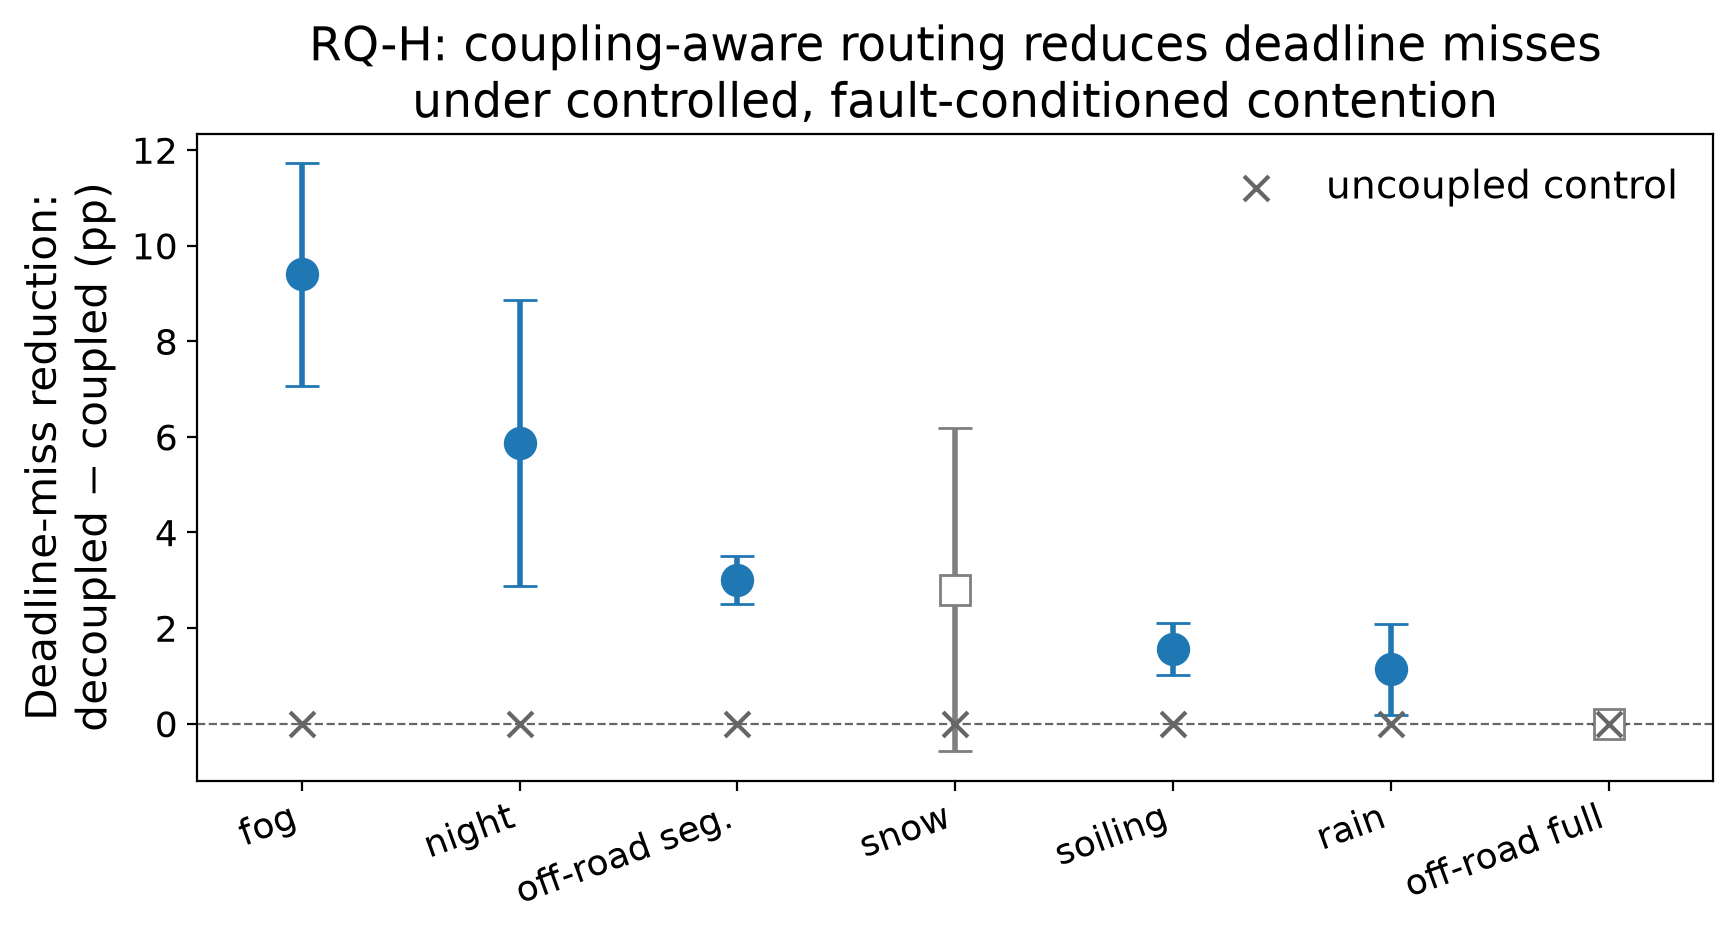
\includegraphics[width=\columnwidth]{fig_rqh_summary.png}
  \caption{RQ-H headline result. Deadline-miss reduction of the
  coupled policy over the decoupled baseline. Filled circles:
  coupled regime, CI excludes zero. Square: CI includes zero. Grey
  crosses: matched uncoupled controls, all exactly $0.0$\,pp. The
  condition-level pattern is more consistent with deadline-binding
  degradation severity than with fault frequency alone.}
  \label{fig:summary}
\end{figure}

\section{Related Work}
\label{sec:related}

TartanDrive \cite{triest2022tartandrive} and TartanDrive~2.0
\cite{sivaprakasam2024tartandrive2} provide off-road driving data
over rough terrain. RADIATE \cite{sheeny2021radiate} provides rain,
snow, fog, and night sequences from a vehicle with stereo cameras.
WoodScape \cite{yogamani2019woodscape} contributes fisheye
automotive imagery with soiling annotations, allowing a cross-optics
test.

Fault monitoring and anomaly detection have been studied for
autonomous perception pipelines
\cite{antonante2022monitoring,bogdoll2022anomaly,hou2023fault}.
Stress tests of multi-sensor fusion systems show large accuracy
drops under individual-stream corruption \cite{tian2025fault}, and
RoboDrive benchmarks robustness under sensor malfunctions and
weather \cite{robodrive2024}. Adaptive inference work, including
BranchyNet \cite{teerapittayanon2016branchynet}, edge early-exit
surveys \cite{laskaridis2021adaptive}, and dynamic transformers
\cite{wang2021notallimages}, adapts computation but does not model
sensor fault as evidence about contention. PRAM-R \cite{pramr2025},
AdaFusion-style expert selection \cite{mees2016choosing}, and DynMM
\cite{dynmm} are closer in spirit because they route using
reliability or uncertainty, but they do not estimate compute
contention or test fault-contention coupling.

\section{Method}
\label{sec:method}

We define four inference configurations ordered by accuracy-latency
tradeoff: YOLO11x at image sizes 1280 and 640, and YOLO11n at image
sizes 1280 and 640. Accuracy is IoU-matched per-class detection F1
against the strongest configuration on the same frame. This is
agreement with a reference detector rather than external ground
truth, so systematic reference errors remain a limitation. The
deadline is the median nominal latency of the strongest
configuration. Under contention, that reference configuration becomes
infeasible while cheaper configurations remain feasible.

The frontier is deliberately small. It keeps the routing action space
interpretable and makes the ablation sharp: if the coupled policy
improves deadline behavior, the improvement comes from how the
contention probability is formed, not from a large learned action set.
We still profiled a denser nine-configuration Pareto frontier on fog
as a robustness check. The coupled benefit remains significant there,
although it shrinks because the decoupled policy has better fallback
configurations.

This choice also avoids a common ambiguity in adaptive-inference
papers: whether a policy wins because it estimates system state
better or because its action space contains a lucky operating point.
Here every policy shares the same frontier, deadline, hysteresis
dwell, and per-frame latency table. The only experimental degree of
freedom in RQ-H is the belief transformation used to predict
contention before selecting a configuration.

\begin{figure}[t]
  \centering
  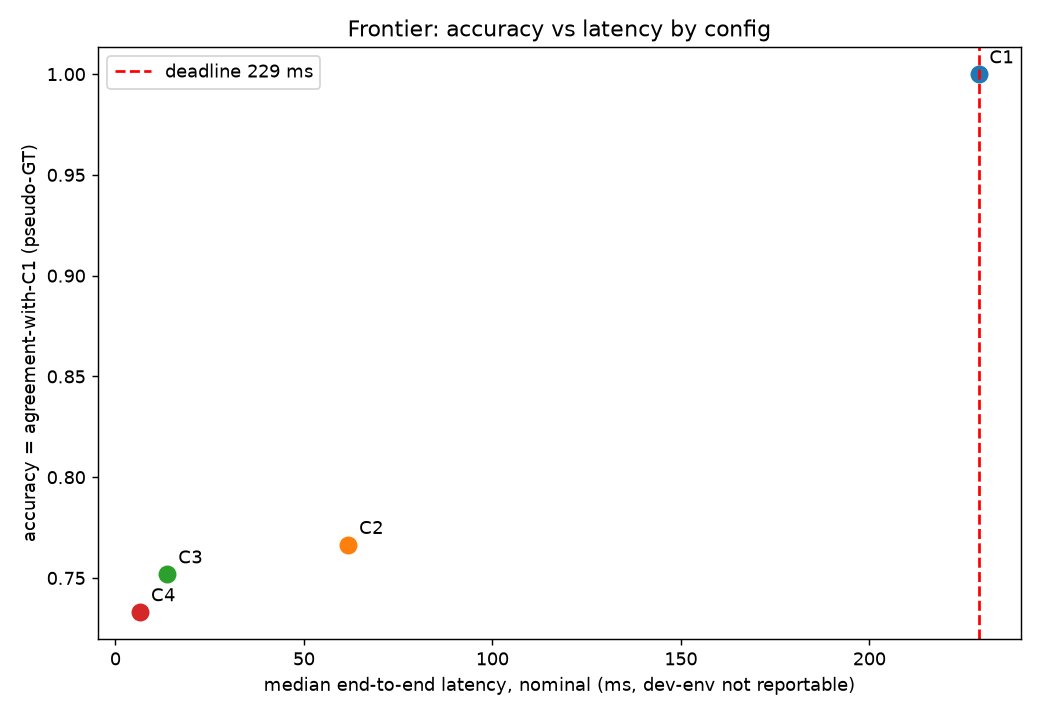
\includegraphics[width=\columnwidth]{fig_frontier.png}
  \caption{Measured accuracy-latency frontier on RADIATE rain. Under
  contention, the reference configuration crosses the self-calibrated
  deadline while cheaper configurations remain feasible.}
  \label{fig:frontier}
\end{figure}

A channel here is one image health signal, not a camera or sensor
modality: we use three, blur, illumination, and occlusion. For each
channel $k$, a four-state switching HMM tracks
$z_k \in \{\text{nominal},\text{degrading},\text{faulted},
\text{recovering}\}$ with Gaussian per-state emissions over the
robust-$z$ normalized signal. For fisheye soiling, occlusion uses
the real soiling-mask pixel fraction rather than optical flow. The
fault belief is
\begin{equation}
  b_f^t = \max_k P(z_k^t=\text{faulted}\mid o_{1:t}).
\end{equation}
Compute contention is a two-state HMM over recent latency features
(p95, p99, and queue depth), producing
$b_c^t=P(z_c^t=\text{contended}\mid \ell_{1:t})$.

\begin{figure}[t]
  \centering
  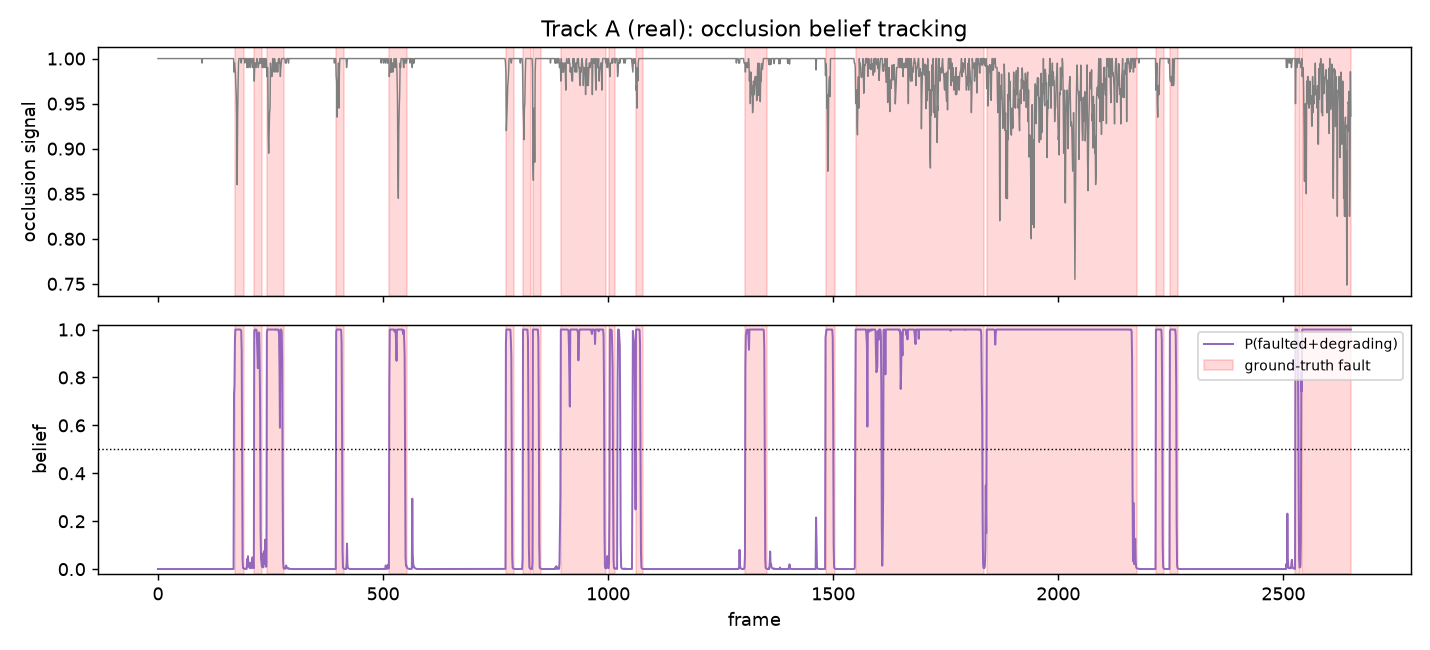
\includegraphics[width=\columnwidth]{fig_belief_occlusion.png}
  \caption{Occlusion fault belief on RADIATE rain. The raw
  track-survival signal is noisy; the switching-HMM posterior
  recovers sustained degradation episodes.}
  \label{fig:belief}
\end{figure}

Contention is observed through latency, not through the injected
schedule itself. The compute HMM therefore has access only to recent
latency statistics, while the coupled router can raise the predicted
contention probability through Eq.~\eqref{eq:noisyor}. This
separation is what makes the decoupled baseline meaningful: it sees
the same beliefs and the same frontier, but it does not use sensor
fault as a predictor of contention.

\begin{figure}[t]
  \centering
  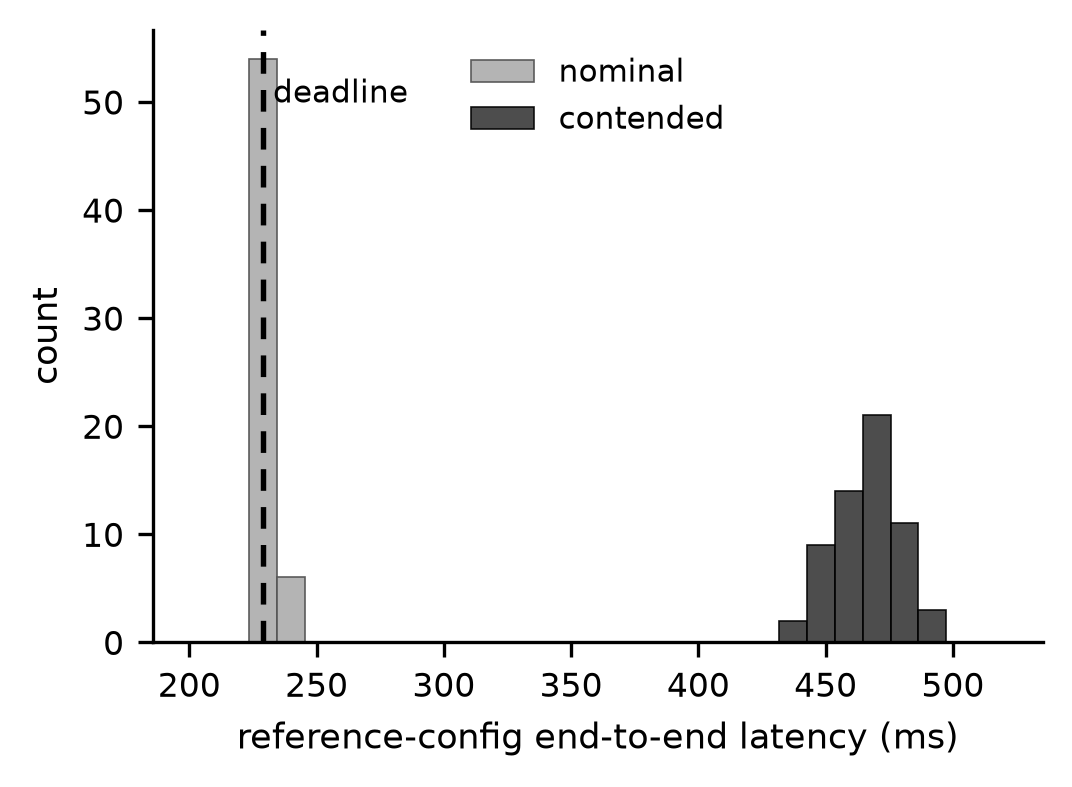
\includegraphics[width=\columnwidth]{fig_contention.png}
  \caption{Reference-configuration (C1) end-to-end latency on
  RADIATE rain, nominal vs.\ contended, with the self-calibrated
  deadline. Induced contention moves the distribution from mostly
  within the deadline to mostly beyond it; the contention probe's
  p95 shift is about $2.5\times$ (Table~\ref{tab:profile}).}
  \label{fig:contention}
\end{figure}

The decoupled policy uses $p_{\mathrm{cont}}^t=b_c^t$. The coupled
policy uses
\begin{equation}
  p_{\mathrm{cont}}^t =
  1-(1-b_c^t)(1-\kappa b_f^t),
  \label{eq:noisyor}
\end{equation}
where $\kappa\in[0,1]$ is fit on a held-out calibration draw from
the same trace, never on the test window. Both policies choose the
highest expected-accuracy configuration whose median latency is
feasible under the predicted compute state. They differ only in the
cross-prediction from sensor fault to contention.

The median-latency feasibility rule is intentionally conservative.
It does not assume that the router can predict each frame's realized
latency; it only asks whether the profiled distribution for a
configuration is appropriate for the current belief state. This
keeps the method implementable on embedded systems where only recent
latency summaries are available online.

\begin{algorithm}[t]
\caption{Coupled belief-space routing at frame $t$}
\label{alg:router}
\begin{algorithmic}[1]
\REQUIRE sensor observations $o_t$, latency features $\ell_t$,
frontier $\mathcal{C}$, deadline $D$, coupling $\kappa$
\STATE Update sensor HMMs with $o_t$ and set
$b_f^t \leftarrow \max_k P(z_k^t=\mathrm{faulted})$
\STATE Update compute HMM with $\ell_t$ and set
$b_c^t \leftarrow P(z_c^t=\mathrm{contended})$
\STATE Set $p_{\mathrm{cont}}^t \leftarrow
1-(1-b_c^t)(1-\kappa b_f^t)$
\FORALL{configuration $c \in \mathcal{C}$}
  \STATE Estimate feasible probability
  $q_c^t \leftarrow
  P(\ell_c \le D\mid p_{\mathrm{cont}}^t)$
  \STATE Score $s_c^t \leftarrow
  E[\mathrm{acc}_c\mid b_f^t]\,q_c^t$
\ENDFOR
\STATE Choose the highest-accuracy $c$ whose median predicted
latency is deadline-feasible; fall back to $\arg\max_c s_c^t$ if no
configuration is feasible.
\end{algorithmic}
\end{algorithm}

\section{Experimental Setup}
\label{sec:experiments}

We evaluate on four groups of traces. Track A is the full
TartanDrive \texttt{turnpike\_afternoon\_fall} sequence
(1{,}198 frames) plus a contiguous 309-frame rough-terrain segment.
The full sequence is a fault-free negative control; the segment has
30.4\% faulted frames. Track B overlays controlled corruptions on
TartanDrive frames and is used only to validate belief-tracker
timing. Track C is WoodScape soiling, with 3{,}303 fisheye frames
after burst collection and 8.1\% faulted frames. Track D uses
RADIATE rain, snow, fog, and night, with 2{,}589--2{,}659 frames per
sequence and fault fractions from 1.9\% (fog) to 44.4\% (rain).

Contention is induced by device-appropriate background load. On
Apple silicon, this is a separate competitor process because Metal
command buffers cannot safely share the inference thread. The
induced p95 latency shift is $1.71\times$ to $2.59\times$ depending
on the trace.

We are explicit about how the coupled schedule is generated, because
this is where a circularity could hide. The schedule is drawn from
the deterministic threshold-and-smooth fault-segment labels, not from
the router's belief. A frame's label is shifted forward by a fixed
onset-to-contention lag of three frames, and contention is then a
Bernoulli draw with probability $P_c(F)$ when the lagged label is
faulted and $P_c(N)$ otherwise (Table~\ref{tab:profile}). The online
router never receives this schedule. It observes only noisy
per-frame health signals, from which the sensor HMM must infer fault
state, and recent latency statistics, from which the compute HMM
infers contention. The schedule and the router's fault belief share
an origin in the same physical degradation, which is the coupling we
set out to study, but they are not the same signal and the
scheduling variable is never a router input. The uncoupled control
replaces this rule with a periodic schedule independent of faults.
The causal claim is correspondingly narrow: when contention is made
to depend on fault onset, anticipating it through fault belief helps;
we do not claim this dependence arises on its own in the field.

\begin{figure}[t]
  \centering
  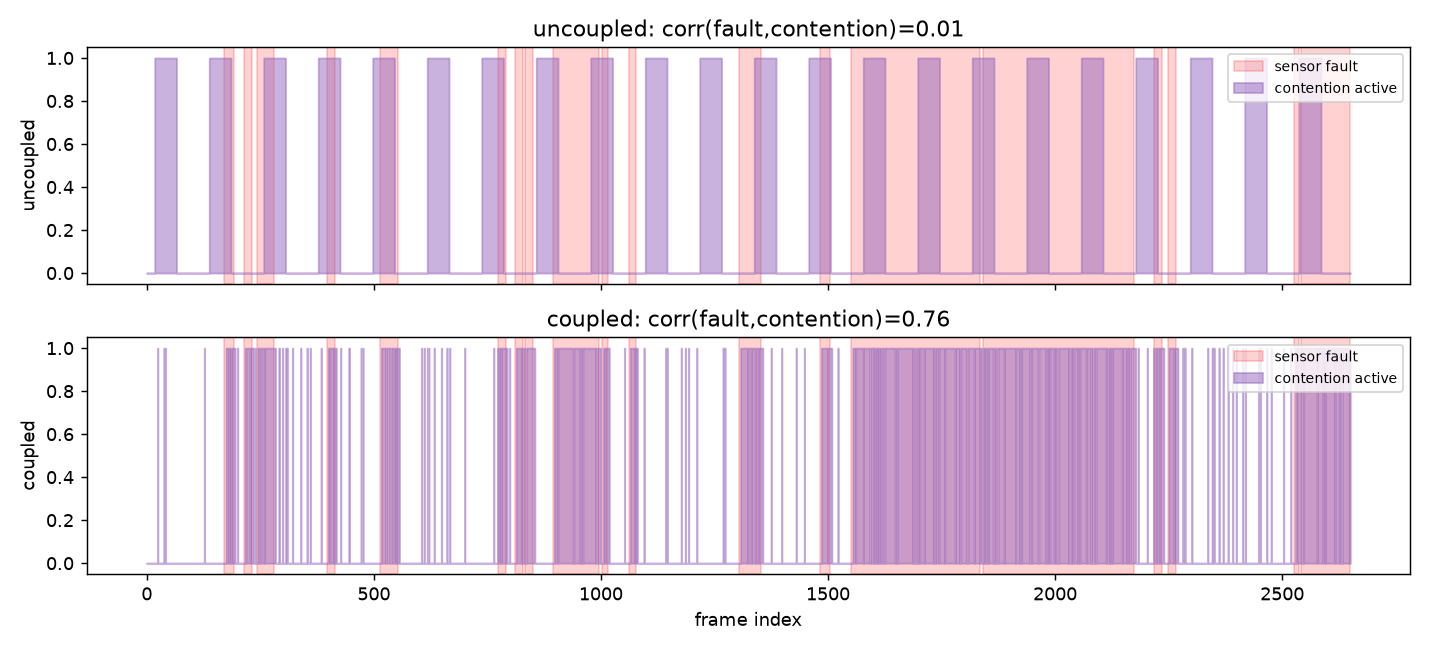
\includegraphics[width=\columnwidth]{fig_regimes.png}
  \caption{Coupled and uncoupled contention schedules on RADIATE
  rain. The coupled schedule is generated from the deterministic
  fault-segment labels, lagged three frames; the router never
  observes it and must infer fault state from noisy signals. The
  uncoupled control uses a fixed periodic schedule independent of
  faults.}
  \label{fig:regimes}
\end{figure}

All experiments run on an Apple~M5 with the Metal backend in fp32.
Absolute latencies are development-environment measurements and are
not the headline result. Each comparison uses five seeds, paired
95\% confidence intervals, and identical frames across seeds; seed
variance comes from injected sensor-measurement noise.

The deadline is calibrated separately for each track from the
profiled reference configuration, so the reported quantity is a
within-device policy comparison. This matters for HPEC-style
reproducibility: another accelerator will have different absolute
latencies, but the same scripts rebuild the local frontier, set the
deadline, rerun the policies, and regenerate the tables. The
repository includes the configuration files, processed outputs, and
scripts used to produce the reported statistics.

The artifact is organized so that reviewers can rerun the paper
without redistributing restricted third-party data. Dataset-specific
scripts construct local manifests from registered copies of
TartanDrive, RADIATE, and WoodScape; subsequent phases cache the
health observations, profile the frontier, generate contention
traces, run the policies, and emit the figures and JSON summaries
used here. The released processed outputs are enough to check the
reported arithmetic, while the acquisition instructions preserve
the original dataset licenses. Table~\ref{tab:params} lists the
parameters needed to reproduce the estimators and statistics; the
full set is in the released \texttt{config.yaml}.

\begin{table}[t]
\caption{Key parameters. The full configuration is released.}
\label{tab:params}
\centering
\scriptsize
\setlength{\tabcolsep}{4pt}
\begin{tabular}{ll}
\toprule
\textbf{Component} & \textbf{Setting} \\
\midrule
Sensor HMM   & 4 states, Gaussian emissions; init stay-nominal \\
             & $0.92$, stay-faulted $0.90$; emission std floor \\
             & $0.30$; transition Laplace smoothing $1.0$ \\
Fault labels & EMA $\alpha{=}0.3$; robust-$z$ threshold $2.5$; \\
             & min segment $5$ frames; recovery hysteresis $8$ \\
Compute HMM  & 2 states; features p95, p99, queue depth over a \\
             & $30$-frame window; init stay-nominal $0.95$, \\
             & stay-contended $0.90$ \\
Accuracy     & IoU $0.5$, confidence $0.25$; per-class F1 vs.\ C1, \\
             & averaged over classes and frames \\
Routing      & hysteresis enter $0.6$ / exit $0.4$, dwell $10$ \\
Coupling     & lag $3$ frames; $\kappa$ fit per trace on a held-out \\
             & calibration draw (seed offset $+100$) \\
Statistics   & $5$ seeds; paired $95\%$ $t$-interval; observation \\
             & noise std $0.15$ (robust-$z$ units) \\
\bottomrule
\end{tabular}
\end{table}

\begin{table*}[t]
\caption{Run profile used for the HPEC submission. Deadlines and
latencies are local Apple~M5/MPS measurements; they define
within-track comparisons rather than portable hardware claims.
$P_c(F)$ and $P_c(N)$ are imposed coupled-regime probabilities of
contention given faulted and nominal frames.}
\label{tab:profile}
\centering
\scriptsize
\setlength{\tabcolsep}{3pt}
\begin{tabular}{lcccccc}
\toprule
\textbf{Condition} & \textbf{Deadline} &
\textbf{C1 p95 nom.} & \textbf{C1 p95 cont.} &
\textbf{Load shift} & \textbf{$P_c(F)$} & \textbf{$P_c(N)$} \\
 & \textbf{(ms)} & \textbf{(ms)} & \textbf{(ms)} &
\textbf{(p95)} & & \\
\midrule
TartanDrive seg. & 237.7 & 244.9 & 525.8 & $1.71\times$ & 0.809 & 0.074 \\
RADIATE rain     & 229.0 & 235.8 & 483.9 & $2.59\times$ & 0.835 & 0.084 \\
RADIATE snow     & 218.5 & 222.6 & 469.1 & $2.57\times$ & 0.775 & 0.067 \\
RADIATE fog      & 217.5 & 219.7 & 461.5 & $2.56\times$ & 0.620 & 0.054 \\
RADIATE night    & 217.2 & 220.6 & 458.6 & $2.54\times$ & 0.794 & 0.058 \\
WoodScape soil   & 341.1 & 353.9 & 718.4 & $2.50\times$ & 0.723 & 0.065 \\
\bottomrule
\end{tabular}
\end{table*}

\section{Results}
\label{sec:results}

We organize the evaluation around two questions. RQ-H asks whether
coupling lowers the deadline-miss rate relative to the decoupled
policy that sees the same beliefs and frontier. RQ-A1 asks whether
persistence-aware belief reduces configuration switching at matched
fault-detection accuracy. Significance throughout is within this
imposed, trace-driven experiment, not a claim about independent
drives or vehicles.

Table~\ref{tab:rqh} and Fig.~\ref{fig:summary} show the main
deadline-miss result. The coupled policy lowers miss rate in every
fault-bearing condition, significantly in five of six. The full
fault-free TartanDrive trajectory has $0.0$\,pp gain, and every
matched uncoupled control is exactly $0.0$\,pp. Fog has the lowest
fault fraction and weakest measured coupling, but the largest
benefit, because its rare episodes are severe enough to make the
reference configuration miss the deadline. Rain faults almost half
the frames but yields only a $+1.13$\,pp reduction.

\begin{figure}[t]
  \centering
  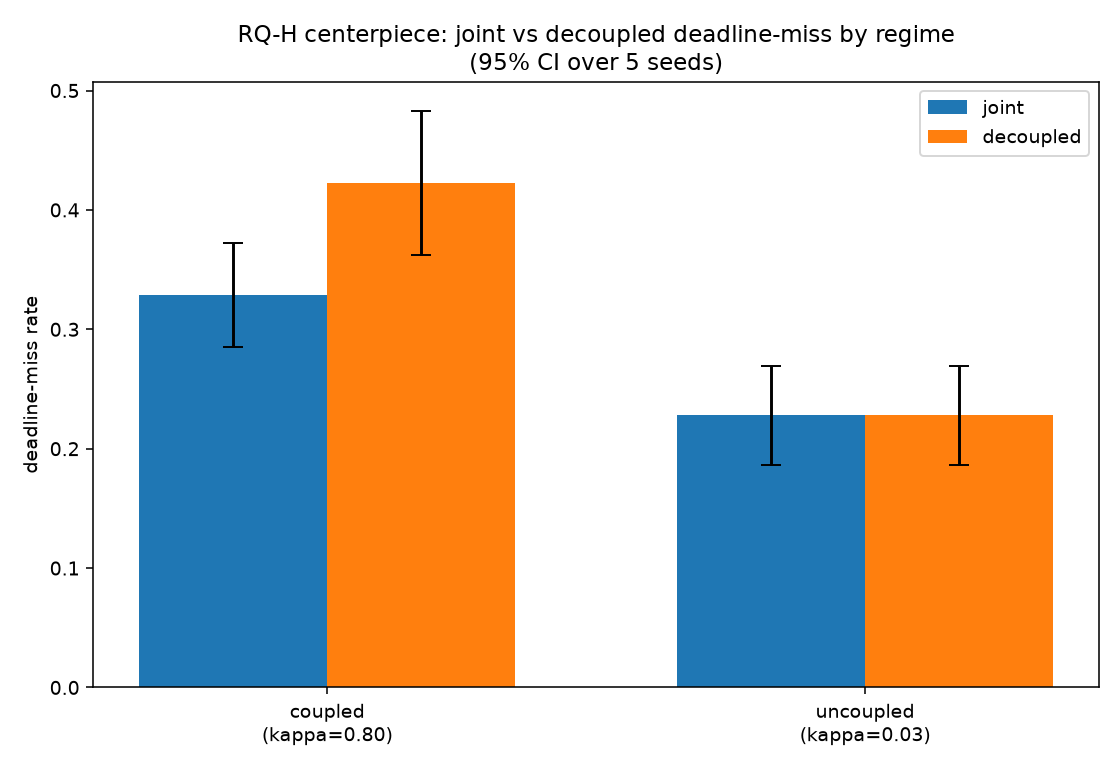
\includegraphics[width=\columnwidth]{fig_rqh_fog.png}
  \caption{RADIATE fog, the strongest RQ-H condition. The coupled
  policy downshifts before rare but severe fog episodes make the
  reference configuration infeasible; the matched uncoupled control
  removes the gain.}
  \label{fig:fog}
\end{figure}

\begin{table*}[t]
\caption{RQ-H. Deadline-miss rate, coupled vs.\ decoupled. $\Delta$
= decoupled $-$ coupled, pp, with 95\% CI. $^\ast$ = CI excludes
zero. $r$ is measured fault-contention correlation in the imposed
coupled regime.}
\label{tab:rqh}
\centering
\scriptsize
\setlength{\tabcolsep}{3.2pt}
\begin{tabular}{llcccccccc}
\toprule
\textbf{Track} & \textbf{Condition} & \textbf{Frames} &
\textbf{Fault \%} & \textbf{$r$} & \textbf{$\kappa$} &
\textbf{Cpl.\ miss} & \textbf{Dec.\ miss} &
\textbf{$\Delta$ (pp)} & \textbf{Uncpl.\ $\Delta$} \\
\midrule
A & TartanDrive full & 1198 & 0.0  & --   & --   & --    & --    & $0.00$ & $0.00$ \\
A & TartanDrive seg. & 309  & 30.4 & 0.74 & 0.79 & 0.249 & 0.279 & $+3.00\ [2.49,3.51]^\ast$ & $0.00$ \\
D & RADIATE rain     & 2651 & 44.4 & 0.76 & 0.80 & 0.233 & 0.244 & $+1.13\ [0.18,2.09]^\ast$  & $0.00$ \\
D & RADIATE snow     & 2589 & 18.5 & 0.69 & 0.82 & 0.313 & 0.341 & $+2.80\ [-0.58,6.18]$      & $0.00$ \\
D & RADIATE fog      & 2659 & 1.9  & 0.31 & 0.80 & 0.329 & 0.423 & $+9.40\ [7.07,11.73]^\ast$ & $0.00$ \\
D & RADIATE night    & 2644 & 12.7 & 0.68 & 0.80 & 0.313 & 0.371 & $+5.87\ [2.87,8.86]^\ast$  & $0.00$ \\
C & WoodScape soil   & 3303 & 8.1  & 0.56 & 0.80 & 0.256 & 0.271 & $+1.56\ [1.01,2.11]^\ast$  & $0.00$ \\
\bottomrule
\end{tabular}
\end{table*}

Deadline miss rate alone can reward aggressive downshifting, so we
also compute on-time utility,
$U=T^{-1}\sum_t a_t\mathbf{1}[\ell_t\le D]$. No tested condition had
a negative point estimate, although three differences were
statistically inconclusive: snow $+1.93$\,pp
$[-0.40,4.25]$, fog $+0.07$\,pp $[-3.65,3.79]$, and soiling
$+0.23$\,pp $[-0.13,0.58]$. The significant utility gains are
off-road $+2.67$\,pp, rain $+0.86$\,pp, and night $+5.87$\,pp.

A hard threshold baseline,
$p_{\mathrm{cont}}=\max(b_c,\mathbf{1}[b_f>0.5])$, performs
similarly to the noisy-OR coupled policy. The coupled-threshold gap
stays within $\pm0.5$\,pp and all CIs include zero. This suggests
that the main contribution is the use of sensor-fault belief for
contention anticipation, not the exact noisy-OR form. A moving-block
bootstrap over time also excludes zero for all six fault-bearing
conditions, including snow, but this checks temporal resampling
within a sequence rather than generalization across independent
drives.

The negative controls are equally important. In the fault-free
TartanDrive full sequence, there is no sensor event from which the
coupled router can anticipate contention, so the coupled and
decoupled decisions coincide. In the matched uncoupled schedules,
faults remain present but the contention process no longer depends
on their onset; the measured RQ-H gain again collapses to zero.
Those two controls separate the coupling effect from a generic
preference for cheaper models.

Because the deadline equals the reference configuration's median
nominal latency, a skeptical reader may worry that this operating
point is chosen to favor the method. Table~\ref{tab:deadline} sweeps
the deadline around each track's calibrated value. The pattern is
consistent across conditions: at $0.8$--$0.9\times$ every policy must
downshift and the advantage is zero everywhere; at the calibrated
$1.0\times$ it is largest; at $1.1$--$1.2\times$ late frames are
rarer and the gap shrinks but stays significant for four of six
conditions. The benefit is therefore concentrated near, but not
confined to, the point where the reference configuration is
borderline feasible. Sweeping $\kappa$ on fog gives a graded
response: $0.0$\,pp at $\kappa=0$, $+3.0$ at $\kappa=0.5$, $+9.3$ at
$\kappa=0.75$, and $+10.9$ at $\kappa=1.0$.

\begin{table}[t]
\caption{Deadline-strictness sweep. Coupled$-$decoupled deadline-miss
reduction (pp) as the deadline is scaled around each track's
calibrated value. $^\ast$ = 95\% CI excludes zero. The benefit peaks
near the calibrated deadline and shrinks, but does not always vanish,
as the deadline loosens.}
\label{tab:deadline}
\centering
\scriptsize
\setlength{\tabcolsep}{3.5pt}
\begin{tabular}{lccccc}
\toprule
\textbf{Cond.} & \textbf{$0.8\times$} & \textbf{$0.9\times$} &
\textbf{$1.0\times$} & \textbf{$1.1\times$} & \textbf{$1.2\times$} \\
\midrule
TartanDrive seg. & 0.0 & 0.0 & $+3.0^\ast$ & $+2.5^\ast$ & $+2.5^\ast$ \\
RADIATE rain     & 0.0 & 0.0 & $+1.1^\ast$ & $+0.5^\ast$ & $+0.5^\ast$ \\
RADIATE snow     & 0.0 & 0.0 & $+2.8$      & $+0.9$      & $+0.9$ \\
RADIATE fog      & 0.0 & 0.0 & $+9.4^\ast$ & $+0.7$      & $+0.7$ \\
RADIATE night    & 0.0 & 0.0 & $+5.9^\ast$ & $+1.9^\ast$ & $+1.9^\ast$ \\
WoodScape soil   & 0.0 & 0.0 & $+1.6^\ast$ & $+0.5^\ast$ & $+0.5^\ast$ \\
\bottomrule
\end{tabular}
\end{table}

\begin{figure}[t]
  \centering
  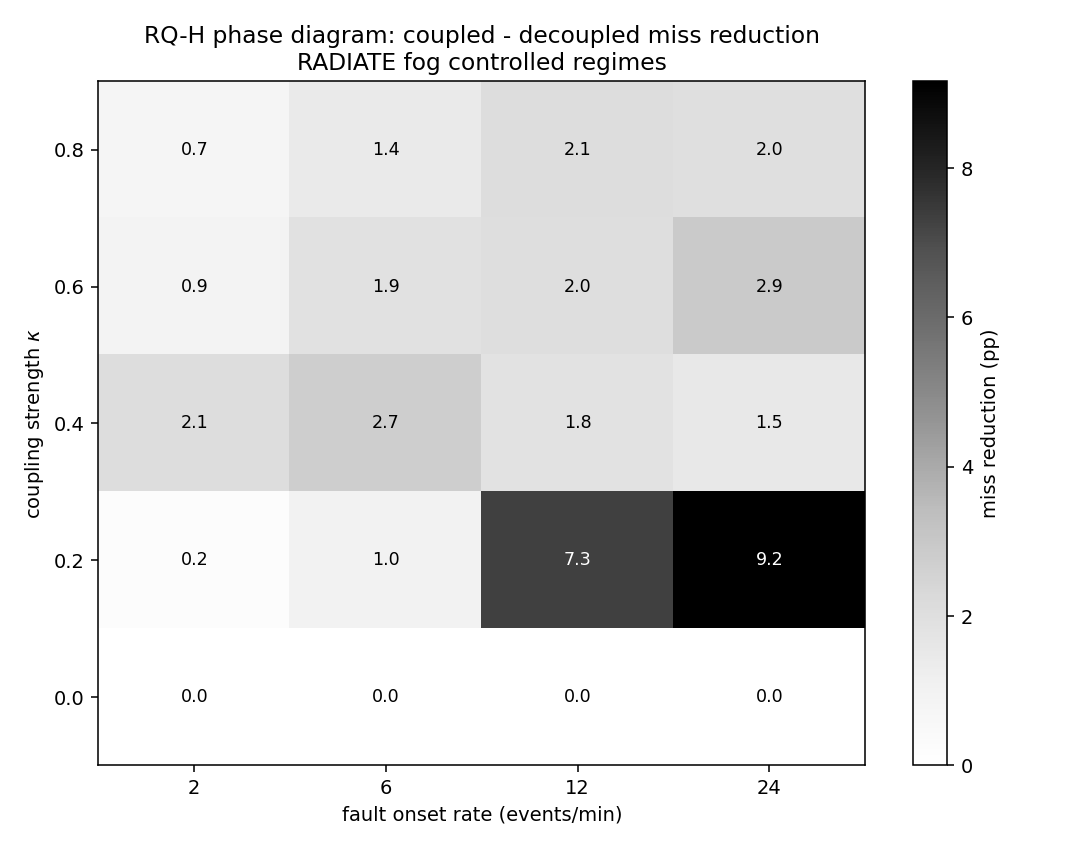
\includegraphics[width=\columnwidth]{fig_phase_diagram.png}
  \caption{Controlled coupling-strength $\times$ fault-onset-rate
  sweep on RADIATE fog. The no-coupling row is zero; under positive
  coupling, the benefit varies nonlinearly with onset rate and
  coupling strength.}
  \label{fig:phase}
\end{figure}

\begin{table}[t]
\caption{Learned-router audit. A two-hidden-layer MLP ($32$--$16$
units) on the same belief features as the coupled policy, trained on
the first $70\%$ of each trace and evaluated on the last $30\%$.
$\Delta$ = MLP $-$ coupled deadline-miss rate (pp) on that held-out
window. Because the window differs from the full sequence, these
miss rates are not directly comparable to Table~\ref{tab:rqh}; for
example, the rain test window happens to contain no contended misses
for the coupled policy.}
\label{tab:mlp}
\centering
\scriptsize
\setlength{\tabcolsep}{3pt}
\begin{tabular}{lccc}
\toprule
\textbf{Split} & \textbf{Cpl.} & \textbf{MLP} & \textbf{$\Delta$} \\
\midrule
Fog      & 0.164 & 0.167 & $+0.22$ \\
Night    & 0.427 & 0.169 & $-25.78^\ast$ \\
Rain     & 0.000 & 0.311 & $+31.11^\ast$ \\
Snow     & 0.289 & 0.324 & $+3.56$ \\
Soiling  & 0.301 & 0.339 & $+3.79^\ast$ \\
A-full   & 0.340 & 0.204 & $-13.56$ \\
A-seg.   & 0.422 & 0.222 & $-20.00^\ast$ \\
\bottomrule
\end{tabular}
\end{table}

The learned-router audit in Table~\ref{tab:mlp} is mixed: the MLP
has lower miss rate on three splits and higher miss rate on four.
It therefore does not replace the coupled policy as a consistent
baseline, but it does show that the belief features carry useful
signal.

Persistence-aware belief improves fault-detection balanced accuracy
on all fault-bearing tracks and reduces configuration switching for
slow degradations such as fog, night, and soiling. It hurts on rain,
where droplet occlusion flickers too quickly for the HMM's
slow-onset assumption. Model-derived hysteresis responds faster than
fixed hysteresis under non-stationary arrivals (1.6 vs.\ 6.6 frames
of onset-to-reconfiguration lag), but switches about 30\% more often.

\begin{table}[t]
\caption{Persistence-aware belief vs.\ memoryless threshold. Positive
$\Delta$ means the belief policy switches less.}
\label{tab:persistence}
\centering
\scriptsize
\setlength{\tabcolsep}{3pt}
\begin{tabular}{lccccc}
\toprule
\textbf{Cond.} & \textbf{Bel.} & \textbf{Mem.} & \textbf{$\Delta$} &
\textbf{bAcc$_b$} & \textbf{bAcc$_m$} \\
\midrule
Rain   & 0.020 & 0.010 & $-0.010^\ast$ & 0.884 & 0.854 \\
Snow   & 0.043 & 0.031 & $-0.012$      & 0.859 & 0.821 \\
Fog    & 0.037 & 0.047 & $+0.011^\ast$ & 0.752 & 0.668 \\
Night  & 0.050 & 0.074 & $+0.024^\ast$ & 0.825 & 0.794 \\
Soil   & 0.020 & 0.052 & $+0.031^\ast$ & 0.862 & 0.808 \\
\bottomrule
\end{tabular}
\end{table}

\begin{figure}[t]
  \centering
  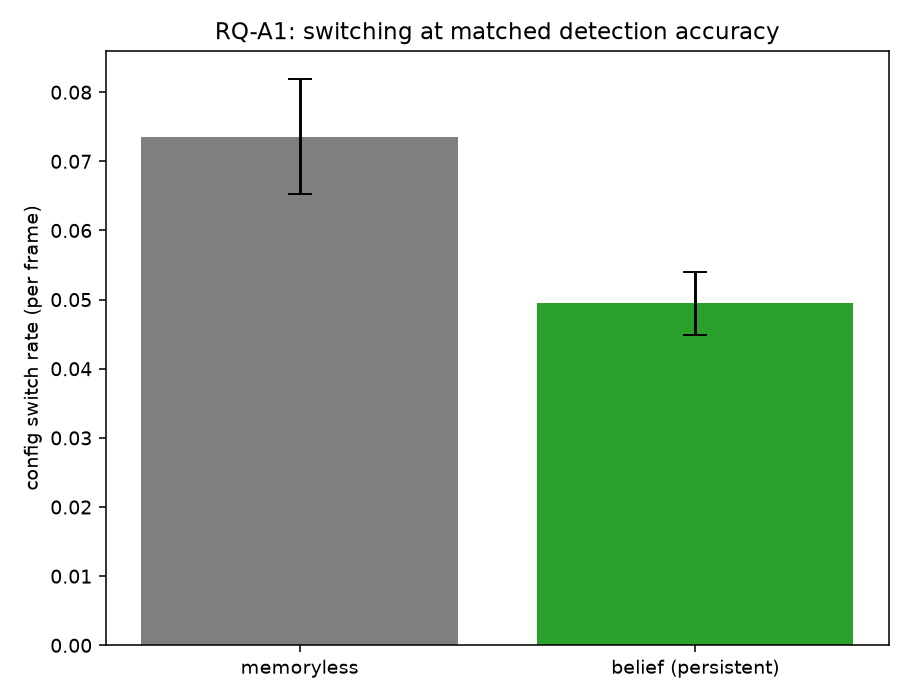
\includegraphics[width=\columnwidth]{fig_rqa1_night.png}
  \caption{RQ-A1 example on RADIATE night. At matched fault-detection
  accuracy, the persistent belief policy switches less often than a
  memoryless threshold, reducing route churn during slow illumination
  degradation.}
  \label{fig:rqa1}
\end{figure}

\section{Discussion}
\label{sec:discussion}

The key scientific claim is narrow. The experiments establish that
when contention is scheduled to depend on fault onset, using
sensor-fault belief to anticipate contention improves deadline
behavior. They do not establish that real deployed robots commonly
exhibit this relationship. The uncoupled controls are therefore
central: they show that the measured benefit switches off when the
fault-contention relationship is removed.

Several limitations remain. The evaluation is offline and
trace-driven, not hardware-in-the-loop. Compute contention is
non-thermal commodity load with a two-state model; embedded systems
can have richer contention. Pseudo-GT is agreement with the C1
reference detector, not external labels. The sensor HMM labels are
derived from health signals that the belief later filters, so fault
validation is partly internal, though Track B provides independent
injection onsets. RADIATE radar, LiDAR, and detection annotations
are not used. WoodScape's temporal order is burst order, not
continuous video. Finally, the five seeds reuse the same frames, so
the CIs measure sensitivity to sensor-measurement noise rather than
generalization across vehicles or routes.

The next step is to replace the imposed schedule with measured
co-occurrence on an embedded platform, for example a Jetson-class
system where perception, planning, and control run together. A full
factorial or cross-coupled HMM could also maintain
$P(z_f^t,z_c^t\mid o_{1:t})$ directly instead of coupling marginal
beliefs only at decision time. Finally, downstream closed-loop tests
should measure task success, not only detector agreement and
deadline misses.

For HPEC readers, the hardware lesson is not that the Apple~M5
latency numbers will transfer to another accelerator. They will not.
The portable claim is procedural: profile the local perception
frontier, estimate whether contention is likely before the latency
tail fully appears, and route to the strongest configuration whose
local distribution satisfies the deadline. The same structure can
also express weaker operational assumptions by lowering $\kappa$ or
by disabling the coupling term when field logs do not show
fault-conditioned load.

The results should also be read as an argument against using fault
frequency alone to prioritize robustness work. Rain faults are common
but often leave a feasible low-cost route, while fog faults are rare
yet deadline-binding in this setup. We do not directly measure
physical degradation severity; we infer its effect from the profiled
frontier and observed deadline misses. A deployment should therefore
log both the health signal and the latency response, then estimate
whether $P(\mathrm{contention}\mid\mathrm{fault})$ is materially
larger than $P(\mathrm{contention}\mid\mathrm{nominal})$ before
enabling the coupling term.

\section{Conclusion}
\label{sec:conclusion}

We built a deadline-aware perception router that estimates
sensor-fault belief and compute-contention belief with separate HMMs
and couples them at decision time. Across real off-road, adverse
weather, and fisheye soiling data, coupling reduced deadline misses
by $1.1$ to $9.4$ points when contention was scheduled to depend on
fault onset. The gain was zero in matched uncoupled controls and on
a fault-free trajectory. The result supports coupled belief-space
routing as a useful mechanism under constructed fault-contention
dependence, while leaving natural field co-occurrence as the next
test.

\bibliographystyle{IEEEtran}
\bibliography{references}

\end{document}
